\documentclass[11pt,aspectratio=169]{beamer}

% ---------------- Theme (safe defaults) ----------------
\usetheme{Madrid}
\usecolortheme{seahorse}
\setbeamertemplate{navigation symbols}{}
\setbeamertemplate{footline}[frame number]

% ---------------- Packages (beamer-friendly) ----------------
\usepackage[T1]{fontenc}
\usepackage{lmodern}
\usepackage{amsmath,amssymb,bm}
\usepackage{graphicx}
\usepackage{booktabs}
\usepackage{xcolor}
\usepackage{listings}
\usepackage{tikz}
\usetikzlibrary{arrows.meta,positioning,shapes,calc}
% ---------------- Graphics path ----------------
\graphicspath{{figs/}} % put images in iv_vae/report/figs/

% ---------------- Listings ----------------
\lstset{
    basicstyle=\ttfamily\small,
    breaklines=true,
    frame=single,
    tabsize=2
}

% ---------------- Title block ----------------
\title[PRML Progress]{Mask-Aware $\beta$-VAE for IV Surface Inpainting}
\subtitle{Progress Report}
\author{Harshil Goyal}
\institute{EE5610: Term Project}
\date{\today}

% ---------------- Handy macros ----------------
\newcommand{\KL}{\mathrm{KL}}
\newcommand{\TV}{\mathrm{TV}}
\newcommand{\E}{\mathbb{E}}

% Placeholder boxes: \ph{width}{height}
\newcommand{\ph}[2]{\fbox{\rule{0pt}{#2}\rule{#1}{0pt}}}
% Quick half-width placeholder: \phh
\newcommand{\phh}{\ph{0.47\linewidth}{1.55in}}
% Quick tall placeholder: \phtall
\newcommand{\phtall}{\ph{0.97\linewidth}{2.1in}}

\begin{document}

% =========================================================
% Title
% =========================================================
\begin{frame}
    \titlepage
\end{frame}

% =========================================================
% Executive Summary (dense)
% =========================================================
\begin{frame}{Executive Summary}
    \textbf{Goal.} Learn a compact latent model (mask-aware $\beta$-VAE) to \emph{reconstruct + inpaint} daily IV surfaces on a fixed $(k,T)$ grid.\\[3pt]
    \textbf{Deliverables (this report).}
    \begin{itemize}
        \item Data bundle (\texttt{.pt}) with $x$, mask, grids, dates
        \item Model + training protocol
        \item Baseline (bicubic)
        \item Result tables + panels
    \end{itemize}
    \textbf{Planned next.} One small ablation ($\beta$ or TV), lightweight no-arbitrage violation counts, final curated panels.
\end{frame}

% =========================================================
% Data & Grid (dense + stats table)
% =========================================================
\begin{frame}{Data \& Grid}
    \begin{columns}[T]
        % ----- Left column -----
        \begin{column}{0.58\linewidth}
            \textbf{Universe.} SPY options (2019--2024).\\
            \textbf{Grid.} $64{\times}64$, $k=\ln(K/S)\in[-0.5,0.5]$, $T\in[7,365]\,$days.\\
            \textbf{Per day.} Field $x\in\mathbb{R}^{64\times64}$, mask $m\in\{0,1\}^{64\times64}$.\\
            \textbf{Norm.} Global min-max on observed cells.\\
            \textbf{Split.} Time-ordered 70/15/15.\\[4pt]
            \vfill
            \begin{center}
                \vspace{-8pt}
                
\includegraphics[scale=0.5]{/home/harshil/IV-Surface-Reconstruction/artifacts/mask_density_over_time.png}
            \end{center}
        \end{column}

        % ----- Right column -----
        \begin{column}{0.42\linewidth}
            \textbf{Dataset stats}\\[-4pt]
            \vspace{4pt}
            \small
            \begin{tabular}{l r}
                \toprule
                Days total         & \, 1508             \\
                Train / Val / Test & \, 1055 / 226 / 227 \\
                Mean obs. frac.    & \, 0.193            \\
                Min/Max obs. frac. & \, 0.096 / 0.251    \\
                IV range (obs)     & \, [0.0115, 1.000]  \\
                \bottomrule
            \end{tabular}
        \end{column}
    \end{columns}
\end{frame}

% =========================================================
% Baseline (bicubic) + pipeline figure
% =========================================================
\begin{frame}[fragile]{Bicubic Baseline: Pipeline}

    \textbf{Bicubic interpolation} on $(k,T)$:
    \begin{itemize}
        \item Fit on observed cells ($m{=}1$)
        \item Eval on mask; report masked-MAE
        \item Fast; classical yardstick
    \end{itemize}
    \vspace{4pt}\centering

    % (Requires: \usetikzlibrary{positioning,arrows.meta})
    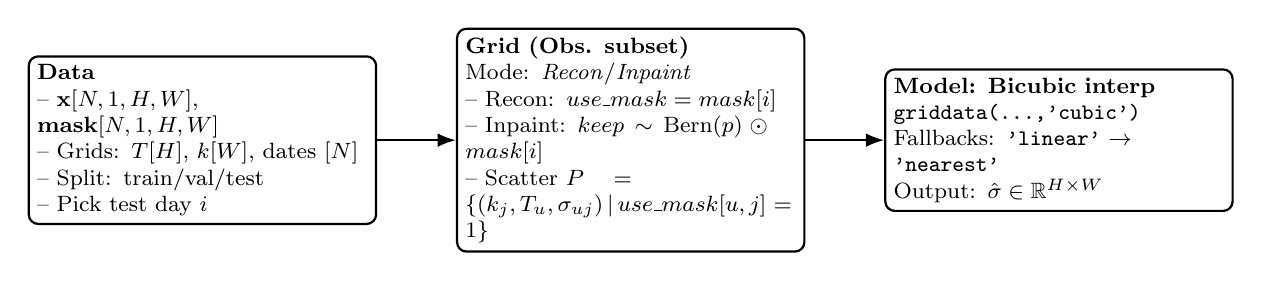
\begin{tikzpicture}[
            font=\footnotesize,
            >=Latex,
            box/.style={draw, rounded corners=1.2mm, thick, align=left, text width=4.2cm, inner sep=3pt},
            line/.style={thick},
            node distance=1.0cm and 1.0cm
        ]
        \node[box] (data) {
            \textbf{Data}\\
            -- $\mathbf{x}[N,1,H,W]$, $\mathbf{mask}[N,1,H,W]$\\
            -- Grids: $T[H]$, $k[W]$, dates $[N]$\\
            -- Split: train/val/test\\
            -- Pick test day $i$
        };

        \node[box, right=of data] (grid) {
        \textbf{Grid (Obs. subset)}\\
        Mode: \emph{Recon}/\emph{Inpaint}\\
        -- Recon: $use\_mask=mask[i]$\\
        -- Inpaint: $keep\sim\mathrm{Bern}(p)\odot mask[i]$\\
        -- Scatter $P=\{(k_j,T_u,\sigma_{uj})\,|\,use\_mask[u,j]=1\}$
        };

        \node[box, right=of grid] (model) {
            \textbf{Model: Bicubic interp}\\
            \verb|griddata(...,'cubic')|\\
            Fallbacks: \verb|'linear'| $\to$ \verb|'nearest'|\\
            Output: $\hat{\sigma}\in\mathbb{R}^{H\times W}$
        };

        \draw[line,->] (data) -- (grid);
        \draw[line,->] (grid) -- (model);
    \end{tikzpicture}
\end{frame}

% =========================================================
% Model (architecture + encoder/decoder figures)
% =========================================================
\begin{frame}{Model: Mask-Aware $\beta$-VAE}
    \textbf{Input (2-channels):} $[x\odot m_{\text{in}},\; m_{\text{in}}]$, where $m_{\text{in}}$ is the full mask for reconstruction or a thinned mask for inpainting.\\[6pt]

    \textbf{Encoder:} Four convolutional layers with strides of 2 and ReLU activations progressively downsample the input from $64{\times}64$ to $4{\times}4$, followed by flattening and two dense layers producing $\mu$ and $\log\sigma^2$ for a latent vector $z \in \mathbb{R}^{16\text{--}32}$.\\[6pt]

    \textbf{Latent Sampling:} $z = \mu + \epsilon \odot \exp(0.5 \log\sigma^2)$, with $\epsilon \sim \mathcal{N}(0, I)$.\\[6pt]

    \textbf{Decoder:} A dense layer reshapes $z$ into $4{\times}4{\times}128$, followed by four transposed convolutional layers with ReLU activations that upsample back to $64{\times}64$, ending with a sigmoid output layer producing $\hat{x}$.\\[6pt]

    \textbf{Loss:} Masked reconstruction loss (MSE) + $\beta$-weighted KL divergence + smoothness and arbitrage regularizers.
\end{frame}

% =========================================================
% Objective (math) + penalty heatmap placeholder
% =========================================================
\begin{frame}{Objective (Masked ELBO + Soft Priors)}
    \small
    \[
        \mathcal{L} =
        \underbrace{\frac{\sum (m^{(\text{loss})}\odot(x-\hat{x})^2)}{\sum m^{(\text{loss})}}}_{\text{masked-MSE}}
        \;+\; \beta\,\KL\!\big(q_\phi(z\!\mid\!x)\,\|\,\mathcal{N}(0,I)\big)
        \;+\; \lambda_{\mathrm{TV}}\TV(\hat{x})
        \;+\; \lambda_{\mathrm{cal}}\,\mathrm{CalMono}(\hat{x}).
    \]
    \vspace{-4pt}
    \[
        \TV(\hat{x}) \approx \sum_{i,j}\sqrt{(\hat{x}_{i+1,j}-\hat{x}_{i,j})^2 + (\hat{x}_{i,j+1}-\hat{x}_{i,j})^2 + \varepsilon},\quad
        \mathrm{CalMono}(\hat{x})=\sum_{i,j} \max\!\{0,\, \hat{\sigma}_{i+1,j}^2 T_{i+1} - \hat{\sigma}_{i,j}^2 T_i\}.
    \]

    \vspace{4pt}
    \textbf{What each symbol means \& why it’s there}
    \begin{itemize}
        \item \textbf{Data \& prediction:} $x\!\in\![0,1]^{H\times W}$ is the normalized IV surface on a fixed grid; $\hat{x}$ is the decoder’s reconstruction.
        \item \textbf{Masking:} $m^{(\mathrm{loss})}\!\in\!\{0,1\}^{H\times W}$ selects the cells used in the loss (observed cells for reconstruction; the hidden subset for inpainting). $\odot$ is elementwise product.
        \item \textbf{Latent model:} $q_\phi(z\!\mid\!x)$ is the encoder’s posterior over latent $z$; the prior is $\mathcal{N}(0,I)$. The $\beta$–scaled $\KL$ term regularizes $z$ (prevents overfit, encourages smoother latents). Typical $\beta\in[1,2]$.
        \item \textbf{TV smoothness:} $\TV(\hat{x})$ penalizes large local gradients across the $(T,k)$ grid (indices $i$ for maturity rows, $j$ for moneyness columns). Small $\lambda_{\mathrm{TV}}$ denoises without washing out structure; $\varepsilon$ prevents division by zero.
        \item \textbf{Soft no-arb (calendar monotonicity):} With total variance $w_{i,j}=\hat{\sigma}_{i,j}^2 T_i$, $\mathrm{CalMono}$ penalizes any decrease along maturity (forward differences $w_{i+1,j}-w_{i,j}<0$). $\lambda_{\mathrm{cal}}$ controls how strictly we enforce time-monotone total variance at each moneyness.
        \item \textbf{Axes \& grids:} $i=1..H$ iterates maturities $T_i$ (from $T_{\min}$ to $T_{\max}$), $j=1..W$ iterates log-moneyness $k_j$ (from $k_{\min}$ to $k_{\max}$).
        \item \textbf{Why masked-MSE:} It makes the objective invariant to how many cells are available and evaluates only where we have ground truth (or where we intentionally hid observations during inpainting).
    \end{itemize}
    \normalsize
\end{frame}

% =========================================================
% Training protocol + curves placeholders
% =========================================================
\begin{frame}{Training Protocol (Implemented)}
    \textbf{Optimizer.} Adam (lr $10^{-3}$, cosine decay), batch 64, $\sim$40 epochs.\\
    \textbf{Curriculum.} Warmup (full recon) $\rightarrow$ inpainting (randomly hide observed cells).\\
    \textbf{Current.} $\beta{=}2$, $\lambda_{\mathrm{TV}}{=}5\times10^{-5}$, $\lambda_{\mathrm{arb}}{=}5\times10^{-3}$.\\[6pt]
    \begin{columns}[T]
        \begin{column}{0.48\linewidth}
            \textbf{Training curves (loss/KL) [Val]}\\
            
\includegraphics[width=\linewidth]{/home/harshil/IV-Surface-Reconstruction/artifacts/val_loss_kl.png}
        \end{column}
        \begin{column}{0.48\linewidth}
            \textbf{Masked-MAE vs epoch [Val]}\\
            
\includegraphics[width=\linewidth]{/home/harshil/IV-Surface-Reconstruction/artifacts/val_masked_mae.png}
        \end{column}
    \end{columns}
\end{frame}

% =========================================================
% Mask curriculum pseudo-code
% =========================================================
\begin{frame}[fragile]{Mask Curriculum (Pseudo-code)}
    \begin{lstlisting}
for epoch in range(E):
    if epoch < warmup:
        m_in, m_loss = m, m
    else:
        keep = Bernoulli(p).sample(m.shape)  # p ~ U(0.2, 0.8)
        m_in   = m * keep                    # hide some observed
        m_loss = m * (1 - keep)              # eval on hidden observed
        if m_loss.sum() < min_obs: m_loss = m

    x_in = concat([x * m_in, m_in], dim=1)
    x_hat, mu, logvar = VAE(x_in)
    L = maskedMSE(x, x_hat, m_loss) + beta*KL(mu,logvar)
        + l_tv*TV(x_hat) + l_cal*CalMono(x_hat)
    step(L)
\end{lstlisting}
\end{frame}

% =========================================================
% Quantitative results tables (you fill)
% =========================================================
\begin{frame}{Quantitative Results}
    \small
    \textbf{Table 1. Reconstruction (observed cells only)}
    \begin{tabular}{lcccc}
        \toprule
        Model                     & Split & Masked-MAE & MSE      & Notes         \\
        \midrule
        Bicubic (baseline)        & Val   & 0.000      & 0.000    & interpolation \\
        $\beta$-VAE ($\beta{=}2$) & Val   & 0.0777463  & 0.010020 & warmup/best   \\
        $\beta$-VAE ($\beta{=}2$) & Test  & 0.075663   & 0.010025 & best ckpt     \\
        \bottomrule
    \end{tabular}

    \vspace{6pt}
    \textbf{Table 2. Inpainting (held-out observed cells)}
    \begin{tabular}{lcccc}
        \toprule
        Model                     & Split & Masked-MAE & MSE      & Notes       \\
        \midrule
        Bicubic (baseline)        & Val   & 0.010020   & 0.000691 & on held-out \\
        $\beta$-VAE ($\beta{=}2$) & Val   & 0.077107   & 0.009935 & on held-out \\
        \bottomrule
    \end{tabular}
\end{frame}

% =========================================================
% Ablation table + plots
% =========================================================
% \begin{frame}{Ablation (one knob; fill numbers)}
%     \small
%     \textbf{Pick one:} $\beta \in \{1,2\}$ \; or \; $\lambda_{\mathrm{TV}} \in \{0, 10^{-4}\}$\\[4pt]
%     \begin{tabular}{lcccc}
%         \toprule
%         Setting                    & Split & Masked-MAE & MSE & Notes \\
%         \midrule
%         $\beta{=}1$ / TV=0         & Val   & --         & --  &       \\
%         $\beta{=}2$ / TV=$10^{-4}$ & Val   & --         & --  &       \\
%         \bottomrule
%     \end{tabular}

%     \vspace{6pt}
%     \textbf{Effect plot (placeholder)}\\
%     \phtall % \includegraphics[width=\linewidth]{ablation_effect_plot.png}
% \end{frame}

% =========================================================
% No-arbitrage checks (heatmaps + counts)
% =========================================================
% \begin{frame}{No-Arbitrage Check (lightweight)}
%     \begin{columns}[T]
%         \begin{column}{0.54\linewidth}
%             \textbf{Violation heatmaps (Before vs After)}\\[2pt]
%             \phh % \includegraphics[width=\linewidth]{violations_before.png}
%             \hfill
%             \phh % \includegraphics[width=\linewidth]{violations_after.png}
%         \end{column}
%         \begin{column}{0.44\linewidth}
%             \textbf{Counts / Fractions (fill)}
%             \small
%             \begin{tabular}{lcc}
%                 \toprule
%                                     & Before & After \\
%                 \midrule
%                 Mean frac. violated & --     & --    \\
%                 Median frac.        & --     & --    \\
%                 95p frac.           & --     & --    \\
%                 \bottomrule
%             \end{tabular}\\[6pt]
%             \textbf{Histograms / CDF}\\
%             \ph{0.9\linewidth}{1.2in} % \includegraphics...
%         \end{column}
%     \end{columns}
% \end{frame}

% =========================================================
% Qualitative panels (dense)
% =========================================================
\begin{frame}{Qualitative Performance}
    
\includegraphics[scale=0.4]{/home/harshil/IV-Surface-Reconstruction/artifacts/qualitative_montage.png}
\end{frame}

% % =========================================================
% % Latent diagnostics (UMAP / t-SNE)
% % =========================================================
\begin{frame}{Next Steps \& Future Prospects}
    \small
    \textbf{Immediate To-Do:}
    \begin{itemize}
        \item Fine-tune hyperparameters and regularizers ($\beta$, $\lambda_{TV}$,
              $\lambda_{arb}$).
        \item Improve mask curriculum and add structured missing patterns.
        \item Add validation metrics (Masked-MAE/MSE, arbitrage violation counts).
    \end{itemize}

    \vspace{2mm}
    \textbf{Model Tweaks (Performance Gains):}
    \begin{itemize}
        \item Larger latent space, residual decoder blocks.
        \item CoordConv inputs and adaptive regularization.
        \item Explore per-cell z-score normalization.
    \end{itemize}

    \vspace{2mm}
    \textbf{Future Extensions:}
    \begin{itemize}
        \item \textbf{CVAE:} Condition on market regime or volatility level.
        \item \textbf{DDPM:} Use diffusion models for stochastic surface generation.
        \item Uncertainty estimation \& cross-asset generalization.
    \end{itemize}

    \vspace{1mm}
    \textit{\footnotesize Note: Further improvements (CVAE/DDPM) may enhance realism but require longer training times.}
    \normalsize
\end{frame}

% =========================================================
% Reproducibility + file map
% =========================================================
% \begin{frame}[fragile]{Reproducibility \& File Map}
%     \textbf{Record:} random seeds, package versions, exact date splits. Save: best ckpt, panels, \texttt{metrics.csv}.\\[4pt]
%     \textbf{File map (example):}
%     \begin{lstlisting}
% iv_vae/
%   report/
%     main.tex
%     figs/                # put your images here
%   src/
%     train_vae.py
%     eval_baseline.py
%     metrics.py
%   artifacts/
%     spy_iv_2019_2024.pt
%     vae_beta.pt
%     panels_*.png
%     results/metrics.csv
% \end{lstlisting}
% \end{frame}

\end{document}
